\documentclass{article}

% Language setting
% Replace `english' with e.g. `spanish' to change the document language
\usepackage[spanish]{babel}

% Set page size and margins
% Replace `letterpaper' with `a4paper' for UK/EU standard size
\usepackage[a4paper,top=1cm,bottom=2cm,left=3cm,right=3cm,marginparwidth=1.75cm]{geometry}

% Useful packages
\usepackage{amsmath}
\usepackage{graphicx}
\usepackage[colorlinks=true, allcolors=blue]{hyperref}
\usepackage{fancybox}
\usepackage{listings}
\usepackage{subcaption}
\lstset{
    language=Matlab,
    extendedchars=true
}

\title{Práctica 2. Optimizar un FSA}
\author{Alvaro Hernandez y André Yermak}
\date{01 de Marzo de 2024}

\begin{document}
\maketitle


%\begin{abstract}
%Your abstract.
%\end{abstract}


\section{Funciones a desarrollar}
El objetivo de esta sección será desarrollar el código necesario para evaluar cómo afecta la longitud de la trama (L, en ranuras) al rendimiento de FSA.

\subsection{Cálculo del rendimiento acumulado}

Para el cálculo del rendimiento acumulado, expresaremos el sistema de ecuaciones para los estados transitorios, vemos que:

%%\[\text{rae} = \lim_{n \to \infty}\frac{1}{N}E[\sum_{k=0}^{n-1}g(X_k)] = \sum_{i=1}^{m} \pi_i g(i)\] %%

\[v_i = \text{g(i)} + \sum_{j=1}^{m}p_{ij}v_j\]

Aquí, $v_i$ representa el rendimiento acumulado en el estado i, g(i) es el promedio de las recompensas por transición en el estado i, y $p_{ij}$ son las probabilidades de transición.

expresándolo en  forma matricial:

\[v = g + Mv \xrightarrow{} v(1-M) = g\]

Una vez expresada la fórmula, la función implementa este cálculo resolviendo el sistema de ecuaciones lineales:

\quad

\begin{verbatim}
%Toma como parametros una matriz M (estados transitorios) y otra g (vector de recompensas).
% Devolvera el vector v.

function v = calcula_rae(M,g) 

    % I será la matriz identidad de las mismas dimensiones que la matriz M
    I = eye(size(M)); 

    % Se llama a F a la resta de (1-M) para usarse en el producto 
    F = I - M;
    
    % Esto sera igual a F*v = g, nos resuelve el sistema de ecuaciones devolviendo v
    v = F \ g ; 
    end
\end{verbatim}

Comprobaremos la función con los datos proporcionados en la práctica:

\begin{verbatim}

>> M = [0.2, 0.3, 0.1; 0, 0.2, 0.4; 0.1, 0.2, 0]; g = [2;4;6];
>> calcula_rae(M,g)

ans =

    7.0504
    9.2806
    8.5612
\end{verbatim}



\subsection{Cálculo del tiempo esperado}

En esta función se calculará el numero esperado de ranuras que transcurren hasta que se transmiten correctamente N paquetes, dado un número L de ranuras por trama. Usaremos L como el vector recompensa al llamar a la función calcula rae.

\begin{verbatim}
function tiempo = calcula_tiempo (N,L)

    % Carga el fichero matrices.m
    load matrices;

    % P usará la propiedad cell de matlab para ser una matriz de matrices.
    P = matrices{N,L};

    % Se elimina la primera fila y columna
    M = P(2:end,2:end);

    % Vector de unos para poder redimensionar el parámetro de entrada L
    g = ones(size(M,1),1);
    g =g*L; 

    % Vector de recompensa acumulada, donde v(n) será el tiempo que devolvamos
    v = calcula_rae(M,g);
    tiempo = v(N); 

end
\end{verbatim}

Comprobaremos la función con los datos proporcionados en la práctica:

\begin{verbatim}
>> calcula_tiempo(10,4)

ans =

   32.9163
\end{verbatim}

\subsection{Cálculo del número de transmisiones}

Para ello, se modificarça levemente el código anterior para tener un vector g con la cuenta de los estados, que dependerá del parámetro introducido N.

\begin{verbatim}
function s = calcula_transmisiones (N,L)

    % Carga el fichero matrices.m y se usa la propiedad cell para hacer
    % una matriz con los índices N y L, que serán también matrices
    load matrices;
    P = matrices{N,L};

    % Se elimina la primera fila y columna de M, y hacemos el vector de recompensa que 
    % en este caso será la cuenta de los estados
    M = P(2:end,2:end);
    g =1:N; 

    % Calculamos la recompensa acumulada y nos quedarmos con la posición que corresponde
    % con la cantidad de filas que tiene la matriz M
    v = calcula_rae(M,g');
    s = v(size(M,1)); 
end
\end{verbatim}

Comprobaremos la función con los datos proporcionados en la práctica:

\begin{verbatim}
>> calcula_transmisiones(10,4)

ans =

   54.6635
\end{verbatim}

\section{Gráficas esperadas}

\subsection{Gráfica del tiempo y de rendimiento}

Para este apartado, se pide emplear la función proporcionada por la práctica \verb|script_graficas()|. Como el código solo renderiza una sola gráfica por valor de N, se ha modificado levemente para que N sea un vector con tres valores (En este caso, hemos puesto N = [10,14,18]) y se usará un bucle con estos tres valores para añadir al "plot" de cada figura, de este modo, salen las tres líneas en la misma gráfica.

\begin{figure}[h]
	\centering
	\begin{subfigure}{0.5\textwidth}
		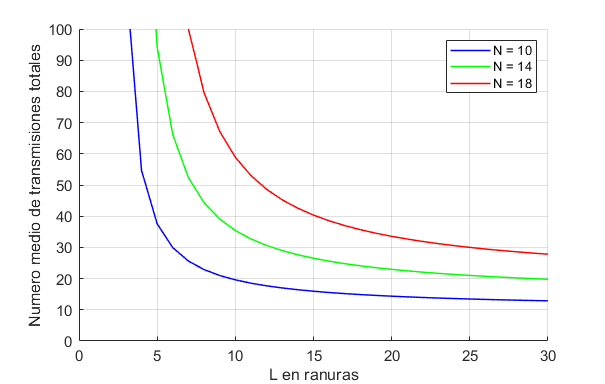
\includegraphics[width=\linewidth]{Transmisiones.png}
		\caption{Transmisiones}
		\label{fig:subfig1}
	\end{subfigure}%
	\begin{subfigure}{0.5\textwidth}
		\includegraphics[width=\linewidth]{tiempo.png}
		\caption{Tiempo}
		\label{fig:subfig2}
	\end{subfigure}
	\caption{Gráficas generadas}
	\label{fig:entire-figure}
\end{figure}


\section{Reto de la práctica}

\subsection{Función de la matriz transición}

El reto que se plantea será:

\quad

Implementar la función \(P = \verb|matriz_transicion(N, L)|\) que calcule la matriz de transición \(P\) a partir de unos valores \(N\) y \(L\) de entrada. Utilice la función \(p\_rx = \verb|p_recepcion(k, n, L)|\) que devuelve la probabilidad \(p\_rx\) de que haya \(k\) paquetes sin colisión en una trama de \(L\) ranuras con \(n\) usuarios activos (es decir, \(p\_rx\) es la probabilidad de recibir \(k\) paquetes de los \(n\) transmitidos).

\quad

Para ello, se recorrerá con dos bucles cada posición de fila y columna en nuestra matriz deseada, que será \textbf{p} en nuestra función. Llamaremos en cada iteración  a la función proporcionada por la práctica  \(\verb|p_recepcion(k, n, L)|\), sabiendo que:
\begin{itemize}
    \item \textbf{k} es el número de paquetes sin colisionar. Es decir, si hay 2 usuarios, pueden existir 0,1 o 2 paquetes sin colisionar que a su vez indica a qué fila nos desplazamos (si no ha colisionado ningún paquete quiere decir que pasamos de tener 2 usuarios a 0 en el siguiente estado)
    \item \textbf{n} es el número de usuarios activos actualmente. Esto coincidirá con las filas de nuestra matriz de transición.
    \item \textbf{L} es el número de ranuras que tenemos, se introduce como parámetro de entrada en la función.
\end{itemize}

Por lo que, sabiendo la teoría de cada parámetro, dependerá de si el número de saltos es mayor que el número de usuarios, algo que físicamente no podría pasar.

\quad

El código en MATLAB será:

\newpage

\begin{verbatim}
function p = matriz_transicion(N,L)

    % Se crea la matriz P de tamaño N+1
    p=zeros(N+1);

    % Como hay que rellenar la matriz con las probabilidades de p_rx, hay que
    % recorrer dicha matriz en ambos ejes, i j con doble bucle llamando a p_recepcion()
    % por cada iteración, siendo que, dependiendo de si el número de saltos es
    % mayor o menor que el número de usuarios, el valor de k como entrada de p_recepción
    % será lo llamado k o la iteración j

    for i=0:(N)
       for j=0:(L-1)
           k=i-j;
           if (k<0)
               p_rx=p_recepcion(j,i,L);
           else
               p_rx=p_recepcion(k,i,L);
           end
         
           p(i+1,j+1)=p_rx;
       end % Fin del primer bucle
    end % Fin del segundo bucle
    p
end
\end{verbatim}

\end{document}